\chapter{Introduction}
% Following the PLoS guidelines, I will use sections, subsections, and paragraphs for my headings.
This thesis focuses on the human microbiome, its relation to human diseases, and techniques used in the data analysis and exploration of it. During the course of my thesis, I conducted one study about non-alcoholic fatty liver disease, one study about atherosclerosis, and written a conference paper about alternate weightings of a common microbiome analysis technique (UniFrac). Each of these topics is represented as a chapter of my thesis.

\section{The human microbiome}
Approximately half of the cells that make up the human body are bacterial (Sender, 2016). Trillions of these bacteria live in the gut (Guarner, 2003), and have a massive metabolic potential. For example, the gut microbiome has been shown to produce changes in hormone levels (Markle, 2013), short chain fatty acid levels (Turnbaugh, 2008), and ethanol levels (Krebs, 1970), to name a few. The human gut microbiome can even digest polysaccharides otherwise unusable by humans (Flint, 2008).

This massive metabolic potential produces measurable symptomatic effects. Transplanting gut bacteria from obese mice to lean mice have been shown to convert lean mice to absorb more calories from the same food (Turnbaugh, 2006). The microbiome can also affect behavior: Completely germ free mice exhibit more anxiety-like behaviors than specific pathogen free mice (Neufeld, 2011).

The human microbiome opens up a host of possibilities for reducing the effects of disease and improving quality of life. However, until recently, a deep understanding of the human microbiome has been beyond the reach of available technology. For example, Escherichia coli is a common model gut bacteria because it is easy to culture, however in reality only makes up about 1% of the average human gut microbiome (Arumugam, 2011).

With the advent of next generation sequencing, scientists can obtain a more comprehensive snapshot of the bacterial composition of the microbiome, what genes they have, and what proteins they produce (Di Bella, 2013). We are in a phase of developing the experiments and accompanying statistical techniques to elucidate the exact mechanisms by which the human microbiome affects health and disease. Armed with a deeper understanding of how the microbiome works, we may be able to develop probiotic techniques to improve quality of life.

\section{Exploring the human microbiome}
The advent of next generation sequencing has prompted the development of a number of different experiments that can be run on biological samples of the human microbiome. Samples can be collected by swabbing the target body site or collecting excretions such as saliva or stool. Products such as DNA or RNA may be extracted as appropriate for the analysis.

Usually a study involves an experimental group and a control group. These can be patients with disease and healthy controls (Macklaim, 2013), people who are susceptible and resistant to a condition (Theriot, 2014), or patients before and after a medical intervention (Graessler, 2013). The questions that scientists in this field generally want to answer are: Is the human microbiome driving or associated with the difference between the two groups? If so, what is the mechanism of action? There are also exploratory studies which try to determine what the core microbiome for a body site in a single condition is by examining what people who fit the condition have in common.

The questions that the data can answer directly are: Is there a statistically significant difference in the microbiome between the control and the experimental groups, in terms of the types of microbes present or the microbial genes present? Do separated groups exist in the data? Are the proportional abundances of certain taxa or genes correlated with each other, or with patient metadata? These questions can be answered by metagenomic experiments and statistical analysis, leading to clues about the larger questions of the mechanism of action.

The two metagenomic experiments that can be done with microbiome next generation sequencing data used in this thesis are gene tag abundance and deep metagenomic sequencing (Riesenfeld, 2004). The tag used for gene tag abundance here is the 16S rRNA gene (Gloor, 2010). The process and resulting data of each experiment is described in the next section, followed by a piece about data analysis and points of failure.

\section{Illumina next generation sequencing platform}
Illumina is a next generation sequencing platform. The Illumina MiSeq machines yields up to 25 million reads of paired end 300 nucleotide sequences, and the Illumina HiSeq machines yield up to 4 billion reads of paired end 125 nucleotide sequences, as stated on the official Illumina website (http://www.illumina.com/systems.html). The sequencing works as follows:

\begin{enumerate}
\item DNA is amplified or fragmented to smaller pieces
\item Adaptors are ligated to the ends of the DNA
\item The DNA is denatured into single strands
\item The DNA washed on a flow cell covered in primers, such that complementary DNA sticks
\item The DNA on the flow cell is replicated to form clusters of identical sequences
\item The DNA is made single stranded again
\item Primers, nucleotides, DNA polymerase, and fluorescently labelled nucleotide terminators are added
\item A camera can detect the fluorescently labelled nucleotide terminators for each added base on each cluster of identical sequences, allowing the DNA to be sequenced.
\end{enumerate}

The Illumina technology has been used for years (Bentley, 2008), and standard protocols exist for library preparation, with kits available commercially.

\section{Gene tag abundance}
Gene tag abundance experiments provide an estimate of the proportion of different types of bacteria in the sample. This can be used to answer questions such as:

\textit{What bacterial taxa make up the microbial community?}
Scientists often want to characterize microbiomes for certain conditions. For example, the core gut microbiome was described by one group to have three enterotypes (Arumugam, 2011), however, when another group studied a diverse population including non-Western people, the enterotypes did not hold (Yatsunenko, 2012). The vaginal microbiome is known to be Lactobacillus dominated, except in bacterial vaginosis, where the microbiome is much more diverse (Hummelen, 2010). The idea is that characterizing the core microbiome is can lead to insight on core functions and how they can be altered when the core microbiome is disrupted.

\textit{Are there any differentially abundant taxa between conditions?}
Some theories of disease progression include the involvement of bacteria as pathogens. Others involve bacteria as probiotics, preventing disease progression. Salient examples include atopic dermatitis where flare-ups are associated with an increase in the proportion of Staphylococcus aureus on the skin (Kong, 2012), and RePOOPulate, a probiotic therapy where 33 microbes cultured from a healthy donor were used to successfully treat symptoms of C. difficile (Petrof, 2013).

Historically, Koch’s postulates have been used to determine if a microbe is a disease-causing pathogen: First, the microbe must be present in all cases of the disease. Second, the microbe must not be present and non-pathogenic in other diseases. Third, if the microbe is isolated in pure culture, it can be used to induce the disease (Koch, 1890). One group has created a modified set of postulates that takes DNA sequencing into account (Fredericks, 1996), which can be applied to differentially abundant taxa detected by gene tag sequencing. However, Koch’s postulates do not account for when the same bacteria can have a very different expression profile in health and disease, such as Lactobacillus iners in bacterial vaginosis (Macklaim, 2013).

\textit{Do samples from different conditions cluster together?}
Sometimes when the data is plotted, there appears to be separation between groups, even if specific taxa are not differentially abundant. One example of this is a study on discordant gut microbiomes between twins in Malawi where one twin has kwashiorkor and the other is healthy (Smith, 2013). In this case the microbiomes diverge the most during treatment with ready-to-use therapeutic food.

\subsection{16S rRNA gene sequencing experiment}
The gene tag chosen throughout this thesis is the gene for the 16S subunit of ribosomal RNA. The 16S rRNA gene is present in all known bacteria and has regions of variability interspersed with regions of high conservation. This allows primers to be made to match the conserved regions, such that the variable regions can be amplified, sequenced, and used to infer taxa. Entire databases exist specifically to match the 16S rRNA gene with taxonomy, such as SILVA (Quast, 2013), the Ribosomal Database Project (Cole, 2009), and Greengenes (DeSantis, 2006).

Specifically, we have been using the 16S rRNA primers from the Earth Microbiome Project protocol (Gilbert, 2014), which amplify the V4 variable region of the 16S rRNA gene. This region was identified by PrimerProspector to be nearly universal to archaea and bacteria (Walters, 2011).

\subsection{Operational Taxonomic Units}
Unlike more distinct species, such as mammalian species, bacterial species are not well defined. Bacterial genomes are highly variable, and regions used to identify bacteria vary in a continuum rather than clusters of similar sequences.

Historically bacteria that are have 97% identity in a variable region are considered to be the same taxa. The 97% cutoff was arbitrarily chosen to best map sequence data to bacterial classifications. This threshold maximizes the grouping of bacteria classified as the same species while minimizing the grouping of bacteria classified as different species. Before sequencing bacterial classification was often done by appearance or by metabolic products, so there are outliers where bacteria classified in the same species are actually genetically very different, or bacteria classified in different genus are genetically very similar.

However, it is difficult to determine how a batch of sequences should be partitioned into groups of 97% identity. One way is to perform a clustering algorithm that optimally partitions the groups and then later assign taxonomic identity by matching the sequences with public databases. Another way is to start off with seed sequences from known bacteria and perform the clustering such that the 97% identity groups are centered on the seed sequences. In any case, the resulting taxonomic groupings are known as Operational Taxonomic Units (OTUs), and are used consistently within the same experiment. While OTUs can be annotated with standard taxonomic names such that results can be compared between experiments, technically the taxonomic groupings used by different experiments are not the same.

\subsection{General protocol and rationale}
The 16S rRNA gene sequencing experiment uses next generation sequencing to estimate the proportional abundance of different bacterial taxa. Samples are extracted and prepared for sequencing, and then the sequenced reads are collated into counts per assumed taxa per sample. The resulting table undergoes statistical analysis.

\paragraph{Pre-sequencing processing}\mbox{}\\
There are several very general steps to the pre-sequencing process:

\begin{figure}[h]
\begin{center}
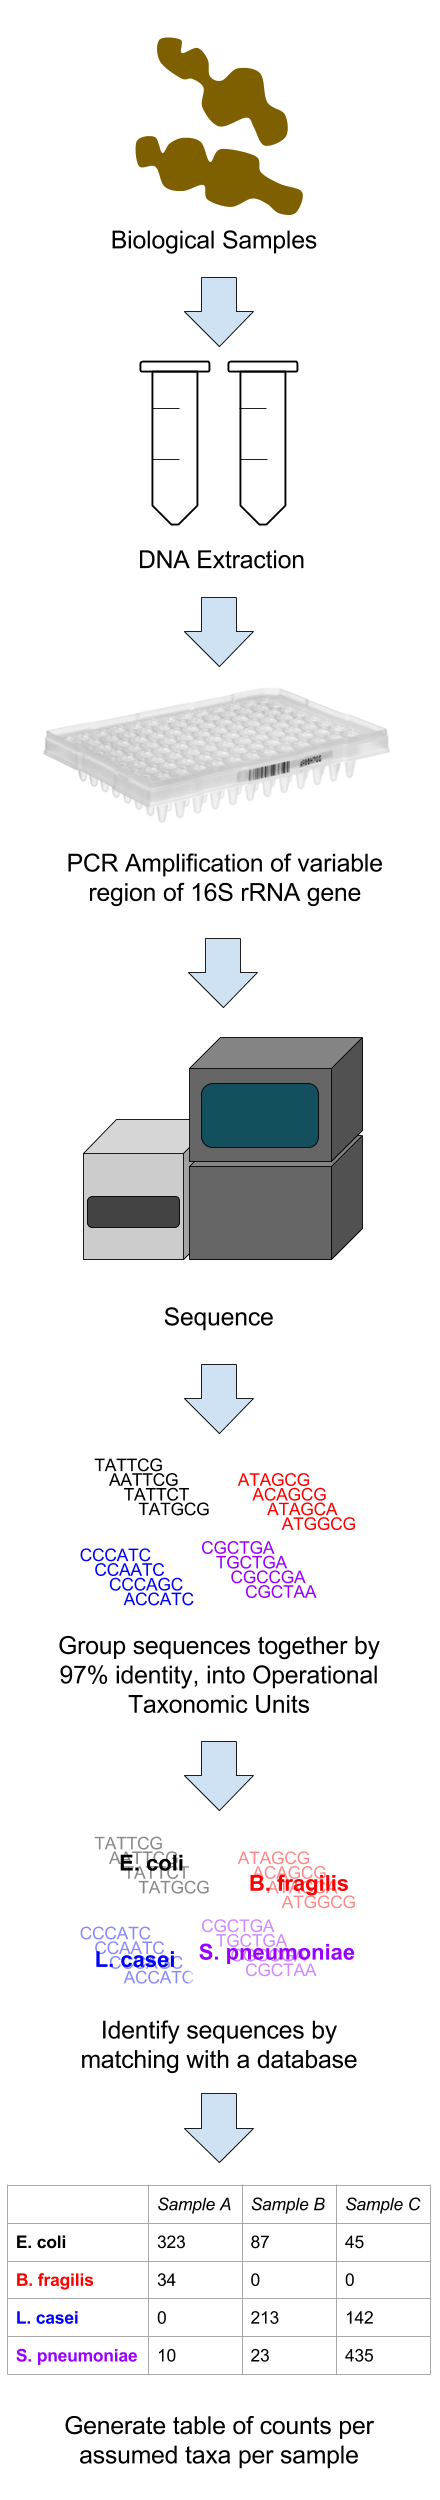
\includegraphics[height=0.8\textheight]{16S_rRNA_pipeline.png}
\caption{A long memory time series\label{ts1}}
\end{center}
\end{figure}

\begin{enumerate}
\item Take a biological sample and extract the DNA
The sample can be collected swabbing the target body site or by collecting samples in some other way. DNA extraction is usually done with common commercial kits.

\item Run a PCR amplification
As discussed previously, the gene tag experiments in this thesis amplify the V4 region of the 16S rRNA gene, following the Earth Microbiome Project protocol (Caporaso, 2012). The set of primers that we use are barcoded, so that we can sequence all the samples in the same sequencing run and differentiate them afterwards.

\item Run sequencing
We use 150 nucleotide paired-end sequencing on the Illumina MiSeq platform. The 150 nucleotide paired ends allow us to overlap paired sequences in the middle to reconstitute the full sequence of the variable region.
\end{enumerate}

\paragraph{Post-sequencing processing}\mbox{}\\
Here are the steps for going from raw sequenced reads to a table of counts per taxa per sample.
\begin{enumerate}
\item Demultiplex the raw sequence
The barcodes are used to separate the sequences according to what sample they came from.

\item Assemble the paired ends of sequenced DNA
The paired sequences are overlapped in the middle, resulting in the full variable region amplified by the primers.

\item Group the reads into operational taxonomic units (OTUs)
We used the mothur software suite to cluster the reads into groups of 97% identity (Schloss, 2009).

\item Annotate the OTUs with bacterial taxonomy
Annotation was done by  matching our OTUs to the SILVA database (Quast, 2013).
\end{enumerate}

Alternatively, an Individual Sequence Unit (ISU) based approach can be taken, where the individual sequences are preserved even after grouping into OTUs, so that different strains within the same OTU can be analyzed separately (Callahan, 2015).

\FloatBarrier

\subsection{Data analysis}
There are two goals in gene tag data analysis. First, is there any structure in the data (separation, clustering, correlations, differentials, etc.)? Second, what drives the structure in the data?

Separation or clustering can be examined by determining the distance between each sample, and using these distances to plot the samples as points on a graph. The following sections will go over the most commonly used distance metric in microbiome research, called UniFrac, as well as the Principal Components Analysis multidimensional scaling method for plotting the points on a graph. Afterwards the data can be visually or mathematically inspected for separation or clustering.

The technique used for determining if taxa are differentially abundant between groups is the same technique used for determining if gene annotations are differentially abundant between groups in the metagenomic experiment, and has its own section, titled “Compositional data analysis”.

\paragraph{UniFrac}\mbox{}\\
Principal Component Analysis is necessary for multivariate statistics, and It is well known that the Principal Component Analysis cannot be performed on proportions, such as the OTU abundances derived from gene tag sequencing. Instead, a Euclidean distance is required (Anderson, 2003).

In 2005, Lozupone et al introduced the UniFrac distance metric, a measure to calculate the difference between microbiomes that incorporated phylogenetic distance (Lozupone, 2005). The goal of UniFrac was to enable objective comparison between microbiome samples from different conditions. In 2007, Lozupone added a proportional weighting to the original unweighted method (Lozupone, 2007). Since then, papers reporting these metrics have garnered over a thousand citations, and enabled research about everything from how kwashiorkor causes malnutrition (Smith, 2013) to how people can have similar microbiomes to their pet dogs (Song, 2013).  Except for Generalized UniFrac, used to make hybrid unweighted and weighted UniFrac comparisons (Chen, 2012), few advances in the metric have occurred since 2007. 

\paragraph{Unweighted UniFrac}\mbox{}\\

\begin{figure}[h]
\begin{center}
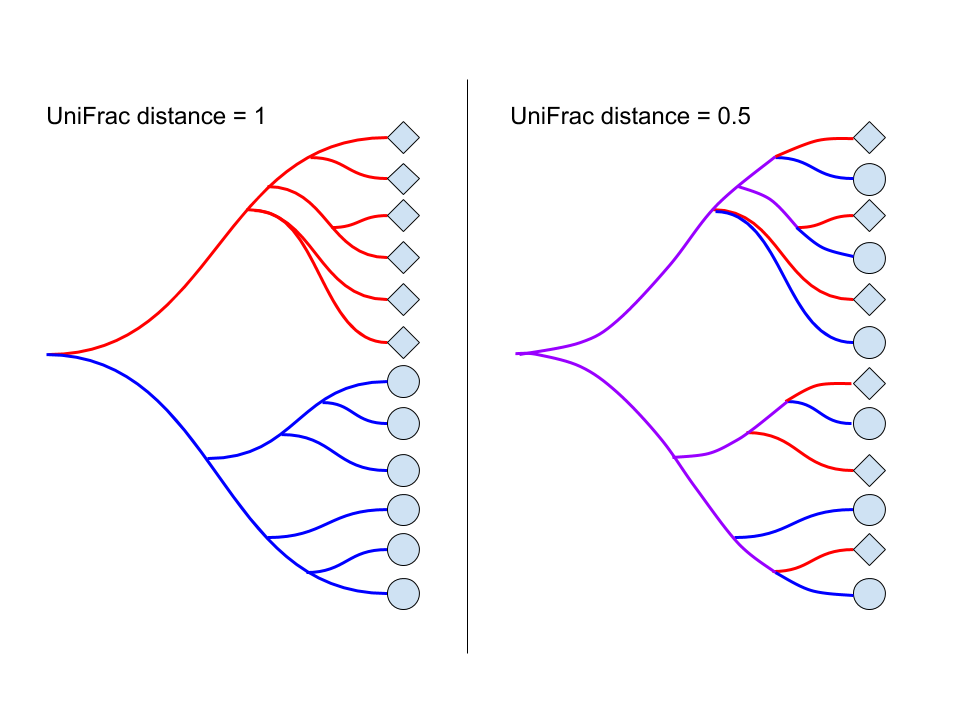
\includegraphics[width=\textwidth]{unifrac.png}
\caption{A long memory time series\label{ts1}}
\end{center}
\end{figure}

Unweighted UniFrac uses an inferred evolutionary distance to measure similarity between samples. It requires a reference phylogenetic tree containing all the taxa present in the samples to be examined. The calculation is performed by dividing the branch lengths shared between the two samples by the branch lengths covered by either sample. A distance of 0 means that the samples have an identical set of taxa detected, and a distance of 1 means that the two samples share no taxa in common.

The qualitative rather than quantitative nature of unweighted UniFrac makes the metric very sensitive to sequencing depth. A greater sequencing depth generally results in the detection of a greater number of taxa. To account for this problem, ecologists use a technique called rarefaction to normalize the sequencing depth across samples by random sampling without replacement (de Cárcer, 2011). However, in unweighted UniFrac samples move relative to the other samples in different rarefaction instances, to the point where they can switch from being a member of one cluster of data to another, as demonstrated in the chapter Expanding the UniFrac Toolbox.

\FloatBarrier

\paragraph{Weighted UniFrac}\mbox{}\\
Weighted UniFrac is an implementation of the Kantorovich-Rubinstein distance in mathematics, also known as the earth mover's distance (Evans, 2012). Rather than looking only at the presence or absence of taxa, each branch length of the phylogenetic tree is weighted by the difference in proportional abundance of the taxa between the two samples. This technique reduces the problem of low abundance taxa being represented as a 0 or by a low count depending on sampling depth. In unweighted UniFrac, such taxa would flip from absent to present, and could skew the measurement: this would be especially problematic if the taxa are on a long branch. In weighted UniFrac, low abundance taxa have a much lower weight and so will have a lower impact on the total distance reported by the metric.

UniFrac is constituted as either a presence/absence (unweighted UniFrac) (Lozupone, 2005), a linear proportion in the form of weighted UniFrac (Lozupone, 2007), or some combination of the two in the form of Generalized UniFrac (Chen, 2012). However, the data are not linear, because the sum of the total number of reads is constrained by the sequencing machinery (Friedman, 2012). Alternative weightings and non-linear transformations of data need to be explored.

\paragraph{Principal Components Analysis}\mbox{}\\
Once the distances between each pair of samples has been calculated, they can be visualized on a plot, with each sample represented as one point. For visualization, the data should be placed so distances are preserved as much as possible, so that clustering and separation of samples can be clearly seen. This is done using the Principal Coordinate Analysis method of multidimensional scaling (Dollhopf, 2001), shortened as PCoA.

To plot all of the samples as points in space such that the distances between each pair of samples are preserved, multiple dimensions are required. In this data specifically, the number of dimensions required is equal to one less than the number of samples. PCoA rescales all the dimensions as components, so that the first component captures the largest variation, or spread of the data, the second component captures the largest variation remaining in the data after the first component, and so on. This way, even if only the first two components are used to plot all the samples as points on a two dimensional graph, the data is spread out to enable visualization of separation or clustering.

After multidimensional scaling the data can be analyzed in several ways. The data can be examined for clustering by k-means analysis (Tibshirani, 2005). The points can also be measured for separation by looking only at their position on the first principal component axis, especially if the first axis covers the majority of the variation in the data set. With each sample associated with a number on the first principal component axis, one can examine the effect size of two different groups by taking the mean positions and dividing by the standard deviation.

\section{The metagenomic experiment}
Deep metagenomic sequencing provides an estimate of the proportion that each type of gene comprises out of the total genes present in the genetic material of the sample. This can be used to answer questions such as:

\textit{What is the metabolic potential of the microbial community?}
The metabolic potential is made up of all the protein functions that are coded by the genetic material present in the sample. Biologically speaking, these protein functions represent the enzymatic reactions that the microbiome could produce if all the genes were expressed. For example, the human gut microbiome has more genes related to methanogenesis, compared to the average sequenced microbe (Gill, 2006).

\textit{Are any genes, functional categories of genes, or metabolic pathways made up of genes differentially abundant between groups?}
In 2006, Turnbaugh et al published a paper showing that an obesity associated gut microbiome in mice had an increased capacity for energy harvest (Turnbaugh, 2006), sparking more research into the gut microbiome and obesity related ailments such as diabetes (Larsen, 2010) and non-alcoholic fatty liver disease (Zhu, 2013). The ability to check if genes, functional categories of genes, or pathways are differentially abundant between groups allows scientists to find clues about the mechanisms by which the microbiome affects certain diseases.

All of this information can be determined by either imputation or actual sequencing, discussed in the next sections.

\subsection{Sequencing}

\begin{figure}[h]
\begin{center}
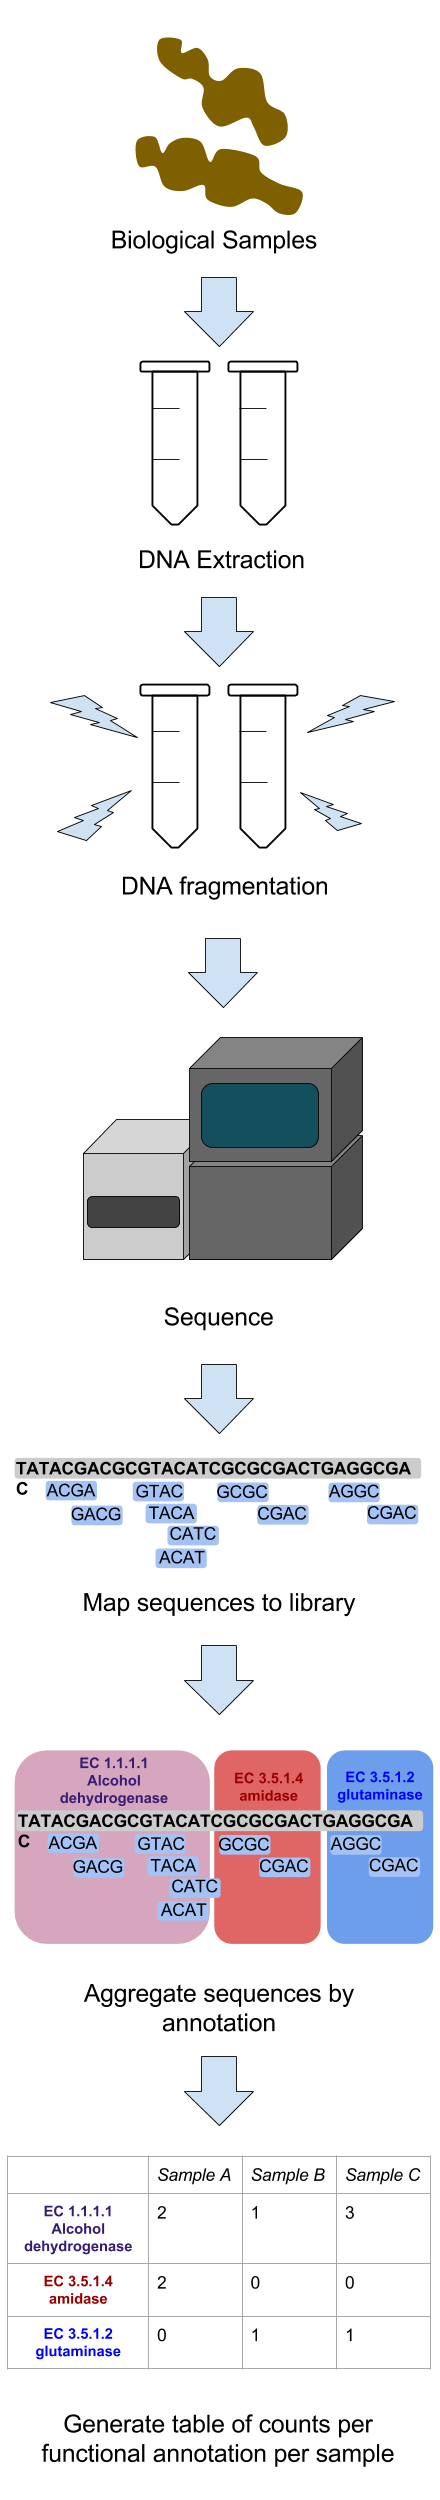
\includegraphics[height=0.8\textheight]{Metagenomic_pipeline.png}
\caption{A long memory time series\label{ts1}}
\end{center}
\end{figure}

The goal of metagenomic analysis is to examine the metabolic potential of the microbiota in the microbiome. This is done by identifying genes, sorting them by the known function of the protein for which they code (such as the catalyzation of a certain reaction), and checking if any functions are differentially present between conditions. Further analysis can also include checking for pathway enrichment, and assembling the sequenced reads into genomes. The general protocol for metagenomic analysis is as follows:

\begin{enumerate}
\item Take a biological sample and perform DNA extraction
The sample can be collected by swabbing the target body site or collecting excretions.

\item Prepare the DNA for sequencing
Fragment the DNA, and filter for the desired size. These steps are all part of the standard Illumina library prep protocol for the HiSeq. There are two options for fragment size, either 50 or 100 nucleotides in length, and we chose the longer one for easier assembly and mapping.

\item Sequence the DNA.
We performed single end sequencing on the Illumina HiSeq platform, with our samples barcoded so that they could be pooled into the same sequencing run.

\item Create an annotated library of reference sequences
The annotated library contains annotations about what kind of protein each sequence codes for. The first step to creating the annotated library is to gather a database of sequences. The database of sequences can be created before the sequencing is complete by gathering all the genomes of all the bacterial strains predicted to be present in the sample, or it can be created after sequencing by assembling the sequenced reads into parts of genomes. The second step is to annotate the sequences with predicted protein functions. Some publically available genomes already have protein annotations. For genomes or partial genomes without annotations, the placement of genes can be predicted by looking for open reading frames, and these predicted genes can be aligned with databases such as SEED (Overbeek, 2005) or KEGG (Kanehisa, 2000) to match them with functional annotations, using the BLAST algorithm (Altschul, 1990).

\item Map the sequenced reads to the library.
Mapping is the process of annotating the sequenced reads by aligning them with sequence that has already been annotated. We used Bowtie2 (Langmead, 2012) to map our sequenced reads to the annotated library created in the previous step. Bowtie2 aligns similar sequences together.

\item Determine how many mapped reads match each functional annotation.
Once the sequenced reads have been mapped to the annotated reference sequence, the number of reads sequenced for each annotation can be counted up. The end result is a table of counts per gene annotation per sample.
\end{enumerate}

Issues with sequencing and the analysis of sequencing data arise from sampling and the fat nature of the data. The sequences that are read by the sequencer are only a small fraction of the DNA from the sample. Additionally, primers used for sequencing may be biased for certain sequences more than others. Lastly, the data is very fat, which is to say that there are magnitudes more variables (in the form of functional annotations of genes) than there are samples. This makes it difficult to have enough power to detect small differences in the data, a concept expanded upon in the Points of Failure section below.

\FloatBarrier

\subsection{Imputation}
Deep metagenomic sequencing can be imputed using a tool called PiCrust from a gene tag experiment (Langille, 2013). PiCrust uses the Greengenes database (DeSantis, 2006) to identify the bacterial taxa in the sample, and pulls their genomes from the Integrated Microbial Genomes database (Markowitz, 2012). With the genomes, the program tries to predict what would be seen if the samples underwent deep metagenomic sequencing. For taxa without a fully sequenced genome, PiCrust infers the genetic content based on ancestors in the phylogenetic tree. PiCrust produces metagenome predictions with Spearman r=~0.7 (Langille, 2013), compared to a full metagenomic sequencing experiment.

Imputation is useful for identifying potential correlations that should be explored and validated further, but should not be used to make conclusions. The issues with imputation include all the issues with sequencing, plus the added variation in its imperfect correlation.

\subsection{Data analysis}
Data analysis can be performed by performed by seeing if functions are differentially abundant between samples in different groups (described in the “Compositional data analysis” section), examining functional categorizations, and checking for pathway enrichment.

\paragraph{Functional categorization}\mbox{}\\

\begin{figure}[h]
\begin{center}
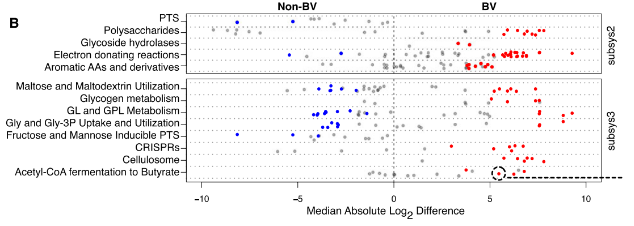
\includegraphics[width=\textwidth]{stripchart.png}
\caption{A long memory time series\label{ts1}}
\end{center}
\end{figure}

We use the SEED annotation, which has four different levels of categorization. Subsystem 4 is the most atomic categorization level and describes the specific function of the protein group, for example, “Isovaleryl-CoA dehydrogenase (EC 1.3.99.10)”. Subsystem 3, 2, and 1 are increasing more general levels of categorizations, from enzyme families to large categorizations such as genes related to carbohydrate metabolism.

Even if the subsystem 4 functional categories are not significantly different between groups, they each have an effect size with a direction. Stripcharts can be used to plot the effect sizes of the subsystem 4 categories for a larger category. For example, by plotting the effect sizes of all the subsystem 4 categorizations under Carbohydrate Metabolism, one can visually see if there are any obvious directional trends for carbohydrate metabolism functions being more present in the experimental group compared to the control.

\FloatBarrier

\paragraph{Pathway enrichment}\mbox{}\\
Biological pathways can be thought of as made up of a series of chemical reactions, each catalyzed by a protein enzyme, which is encoded by a gene. KEGG (Kyoto Encyclopaedia of Genes and Genomes) is a manually curated annotation database that matches genes to pathways (Kanehisa, 2000). This database allows researchers to see if there is differential abundance of pathways encoded by functionally annotated genes, even when the genes may not be differentially abundant by themselves.

\section{Points of failure}
The Huttenhower lab has organized the Microbiome Quality Control project (MBQC) at http://www.mbqc.org/. Preliminary results show that despite being given the same samples, different participating labs can come up with vastly different results. This lack of reproducibility is caused by a lack of consensus on the correct way to analyze microbiome data. The following sections explore different aspects of microbiome data that contribute to this.

\subsection{Collection methods differ}
These experiments are very sensitive to batch effects because microbiome composition can be very variable within groups such that the effect size of a difference between groups can be small. Wherever possible, all samples should be processed in the same batch. Analysis should also be done to check if samples extracted on different dates or sequenced with different primers separate into clusters, to make sure that there is no systematic bias in the data.

\subsection{Microbiome data is highly variable between individuals}
One highly studied body site is the gut, and the gut microbiome can be affected very strongly by diet (Turnbaugh, 2009). This among other factors lead to a highly diverse gut microbiome between subjects for reasons unrelated to the disease being studied, creating a lot of noise, potentially obscuring real effects or even creating the appearance of false effects.

Generally experiments of this nature typically have low sample sizes due to budget constraints, sample collection difficulties, patient compliance, and other issues. To increase cost effectiveness and reduce batch effects, we run all the samples in an experiment on the same sequencing run, by means of a primer design (Gloor 2010).

There are several models for computationally analyzing the variance within conditions in order to determine if operational taxonomic units are significantly differentially abundant, most of which were originally desigend for RNA-seq experiments on single organisms (Pachter, 2011). Currently the most popular tools for analyzing differential abundance are EdgeR (Robinson, 2010), DESeq2 (Love, 2014), and MetagenomeSeq (Paulson, 2014). EdgeR was cited by 1,130 papers in 2015 according to Google Scholar. DESeq2 and MetagenomeSeq are part of the QIIME pipeline, which was cited by 1,620 papers in 2015.

EdgeR and DESeq2 use the negative binomial distribution. The negative binomial distribution allows the variance of data to be estimated given the mean, through a function. The function is determined by collecting the mean and variance for all the counts for each OTU in each experimental condition, and fitting the variances according to the negative binomial distribution. This vastly underestimates the variance at low counts, which represent the sampling of low abundance OTUs, and can be very different between replicates. Underestimating the variance at low counts produces spurious low p-values for low count OTUs (Fernandes, 2013).

MetagenomeSeq uses the Zero-Inflated Gaussian (ZIG) model, which is a binomial distribution of counts (that may include zero counts), plus a function to predict how many extra zeros there will be. This doesn’t work well when the total number of reads are not well matched, because then there will be much more zeros in the data set with less reads, due to having a lower sequencing depth, and a consistent total read count is required between samples according to page 2 of the supplementary material in the first metagenomeSeq paper (Paulson, 2013).

For my differential abundance analysis, I’ve used ALDEx2, which samples from the Dirichlet distribution to model variation in the data (Fernandes, 2014). After a number of samples, the mean value and mean variance are used to determine if OTUs are differentially abundant between groups, an approach that is believed to result in greater sensitivity and equivalent specificity compared to the DESeq2 approach (Fernandes, 2014).

\subsection{Microbiome data involves the comparison of many features}
Oftentimes, the number of taxa or gene functions comparisons is a magnitude larger than the sample size. This is known in statistics as having more variables than observations, or having fat data. The higher the ratio of variables to observations are, the less likely the principal components analysis is to be reliable (Osborne, 2004).

Researchers should include multiple test corrections to ensure that the results they are reporting are true, at the expense of having p-values less than 0.05. Unfortunately many studies have been published in high impact journals without multiple test corrections, including a famous paper linking the gut microbiome to autism published in Cell (Hsiao, 2013).

\subsection{Microbiome data is compositional}
There are several core truths about microbiome data that should be considered when making an analysis strategy.

First, the total number of reads per sample is irrelevant to the biological implications of the data, as it is limited by how the samples were processed and the sequencing platform. Based on spurious correlations discovered in organ size research, it is known that given compositional data (such as bone lengths as a proportion of height, or OTU abundances that add up to the total number of counts per sample), analysis with the assumption that the variables (bone lengths or OTU counts) are independent lead to spurious positive correlations (Pearson, 1896). The variables thought to be independent are related by the sum they are divided by. Additionally, the constrained sum causes the abundance of different taxa to appear to be negatively correlated with each other when analyzed by conventional statistics. When one taxa increases in abundance, the counts detected in other taxa decrease in abundance, even if the taxa are not decreasing in abundance biologically.

Second, removing an entire variable (an OTU in gene tag sequencing, or a functional annotation in deep metagenomic sequencing) from the analysis should not change correlations between OTUs. Removing variables occur routinely in microbiome research, such as when rare OTUs are discarded. Without a data transformation, removing variables will change the correlation between variables (Aitchison, 1986).

To ensure that these conditions are met, data should be analyzed in a compositional way. Several types of log ratio data transformations are recommended to allow the data to be analyzed by standard Euclidean methods (Aitchison, 1986). The type that makes the most sense for microbiome data is the centered log ratio transform. The centered log ratio transform is performed by dividing each proportional abundance by the geometric mean of all the proportional abundances, and taking the logarithm. The geometric mean acts as a low level baseline abundance in microbiome data. Taking the logarithm of the ratio allows for a consistent measurement whether the large number is in the numerator or denominator of the ratio.

The centered log ratio transform prevents the total number of reads from affecting the measurement, so long as the geometric mean is a stable baseline, a condition met in a typical microbiome data set [CITATION NEEDED]. The centered log ratio transform also allows for coherent subcompositional data analysis as remaining values are not affected when entire variables are removed.

Compositional techniques such as those espoused in the Analysis of Composition of Microbiomes (ANCOM) framework (Mandal, 2015) and the ANOVA-Like Differential Expression 2 (ALDEx2) software (Fernandes, 2014) should be used to prevent spurious correlations and promote consistent data analysis. However, these techniques are not yet mainstream in the field.

\subsection{Microbiome data is sparse}
One of the fundamental challenges in analyzing differential abundance is accounting for zeroes. Unlike a presence/absence test, a zero does not necessarily mean that the expression is not there. The expression could be present in an amount smaller than the resolution of the test. This is a problem because when statistical methods are used to examine significantly different expression, the comparison of zero values to non-zero values are likely to come out as significant whether or not the expression is differential. Additionally, the log transformations used in compositional data analysis cannot be performed on zeros.

Two methods have been suggested in the literature to account for zeros. The first is simply to add a small arbitrary value to each zero, as suggested in the original literature about the statistical analysis of compositional data (Aitchison, 1986). This is used in ALDEx2, and the arbitrary value is chosen to be 0.5, representing complete uncertainty in whether or not a zero count in one sample (where the OTU or gene has non zero counts in other samples) would be a 0 or a 1 in a technical replicate (Fernandes, 2013).

The second method is to take a Bayesian approach where the likelihood that a zero could be changed to a positive count if the sample were resequenced is estimated, based on . This is implemented by the cmultRepl command in the zCompositions package in R (Palarea-Albaladejo, 2015). Based on the shape of the rest of the data for the same sample, the average value of the count detected if a zero were resequenced is determined, and the zeros are all replaced by this fraction.

The microbiome field is quite new, and has been undergoing many exciting developments. Gold standards must be set to ensure that studies are replicable, and that published research represents the biological reality.

\section{The gut microbiome in atherosclerosis-susceptible and atherosclerosis-resistant patients}

\section{The gut microbiome in patients with non-alcoholic steatohepatitis compared to healthy controls}












Here is a picture of a long memory time series. 
\begin{figure}[ht]
\begin{center}

\includegraphics[height = 9cm, width = 9cm]{pic1.jpeg}
\caption{A long memory time series\label{ts1}}
\end{center}
\end{figure}

Here's a table.
\begin{table}[ht]
\begin{center}
\begin{tabular}[ht]{|c|lr|c|} 
%c stands for centre, l for left, r for right; the | puts lines in between, and the hline puts a horizontal line in
\hline
$n$ & $\alpha$ &$n\alpha$ & $\beta$\\
\hline
1 & 0.2 & 0.2 & 5\\
\hline
2 & 0.3 & 0.6 & 4\\
\hline
3 & 0.7 & 2.1 & 3\\
\hline
\end{tabular}
\caption{A random table \label{tab1}}
\end{center}
\end{table}

\begin{eqnarray}
y &=& mx + b \label{eq1}\\
&=& ax+ c
\label{eq2}
\end{eqnarray}

This is an un-numbered equation, along with a numbered one. 
\begin{eqnarray}
u &=& px \nonumber\\
p &=& P(X=x) \label{eqn3}
\end{eqnarray}

Look at Table \ref{tab1} and Figure \ref{ts1} and equations \ref{eq1},  \ref{eq2}, and \ref{eqn3}.

Let's do some matrix algebra now.

\begin{equation}
det\left(\left|\begin{array}{ccc} 2 & 3 & 5\\
4 & 4 & 6\\
9 & 8 & 1
\end{array}\right|\right) = 42
\end{equation}

In the equation and eqnarray environments, you don't need to have the dollar sign to enter math mode.

\begin{eqnarray}
\alpha = \beta_1 \Gamma^{-1}
\end{eqnarray}

This is citing a reference ~\cite{mygood11111}.  This is citing another ~\cite{mrx05}.  Nobody said something ~\cite{Nobody06}.
